\chapter{Methodology}
Winning tickets are highly sparse and therefore represent a performant yet reduced form of a function.
Due to their sparsity, the structure of the network may contain useful insights about its functionality.
Analyzing the structure of a network graph, however, is quite challenging.
A different approach would be to use data with a known structure and test if the resulting sparse lottery ticket resembles that structure in any way, as in \autocite{BIMT}.

The following research question was formulated for this thesis:

\begin{quote}
\textit{``Does a lottery ticket that was trained on a dataset with two independent tasks contain two independent subnetworks?''}
\end{quote}

Concretely, for the scope of this thesis, subnetworks derived with iterative magnitude pruning and parameter resetting are examined.
The semantic structure of data can be quite complex.
Therefore, in this thesis, a fundamental semantic structure will be at the center of the investigation: Independence.
Inspired by experiments from in \textcite{BIMT}, two dataset that contain independent tasks are created.

In this chapter, the tools, algorithms, and dataset are described in detail.
First, the software stack is briefly mentioned.
Then, the creation of the Moons-Circles dataset is described, which contains two independent tasks.
Subsequently, the network architecture, related hyperparameters, and the training procedure are outlined.
Following, the methods used for analyzing whether the networks separated and the process of network extension are discussed.
Finally, the creation of the MNIST-Fashion-MNIST datset, a larger dataset containing independent tasks, is explained.

\section{Software Stack}
All software developed within the scope of this thesis is written in Python~\autocite{python}.
Several freely available Python packages are used.
PyTorch~\autocite{pytorch}, a commonly used machine learning library, is used to define neural networks and train them.
NetworkX~\autocite{networkx}, a well-known library for working with mathematical graphs, is used to transform the PyTorch model into a directed graph and analyze it.
Scikit-Learn~\autocite{sklearn} which is also a popular machine learning library, is used to generate the Moons-Circles dataset.
Torchvision, a package related to PyTorch is employed to generate the MNIST-Fashion-MNIST dataset.
Matplotlib~\autocite{matplotlib} is used to generate the plots to visualize the results of the experiments.
Numpy~\autocite{numpy}, a package to work with matrices in Python, provides crucial functionality throughout this thesis to manipulate vectors and matrices.

\section{The Moons-Circles Dataset}\label{sec:independece_dataset}
\textcite{BIMT} executed the experiments on symbolic regression datasets.
These are simple toy datasets where the labels are computed with a symbolic formula. 
For instance regarding the independence task, the inputs are $x_1, x_2, x_3, x_4$ and the outputs are $y_1={x_2}^2 + \sin{(\pi*x_4)}$ and $y_2={(x_1+x_3)}^3$.
In this case, the independence is obvious, as $y_1$ depends only on $x_1$ and $x_3$, and $y_2$ depends only on $x_2$ and $x_4$.
However, concerning lottery tickets, the existing literature focuses on classification tasks, while this is a regression task.
Therefore instead of using the independence dataset from \autocite{BIMT}, a classification dataset with independence is created.
Two classic toy datasets are concatenated into one dataset.
The two selected datasets are the Two-Moons dataset and the Circles dataset, depicted in figure~\ref{fig:moons_circles}.
Both datasets can be interpreted as a two-dimensional plane, where the inputs describe the coordinates of points on the plane. 
The labels of the dataset relate to the class.
Each point belongs to one class: red or blue.

\begin{figure}[ht]
    \centering
    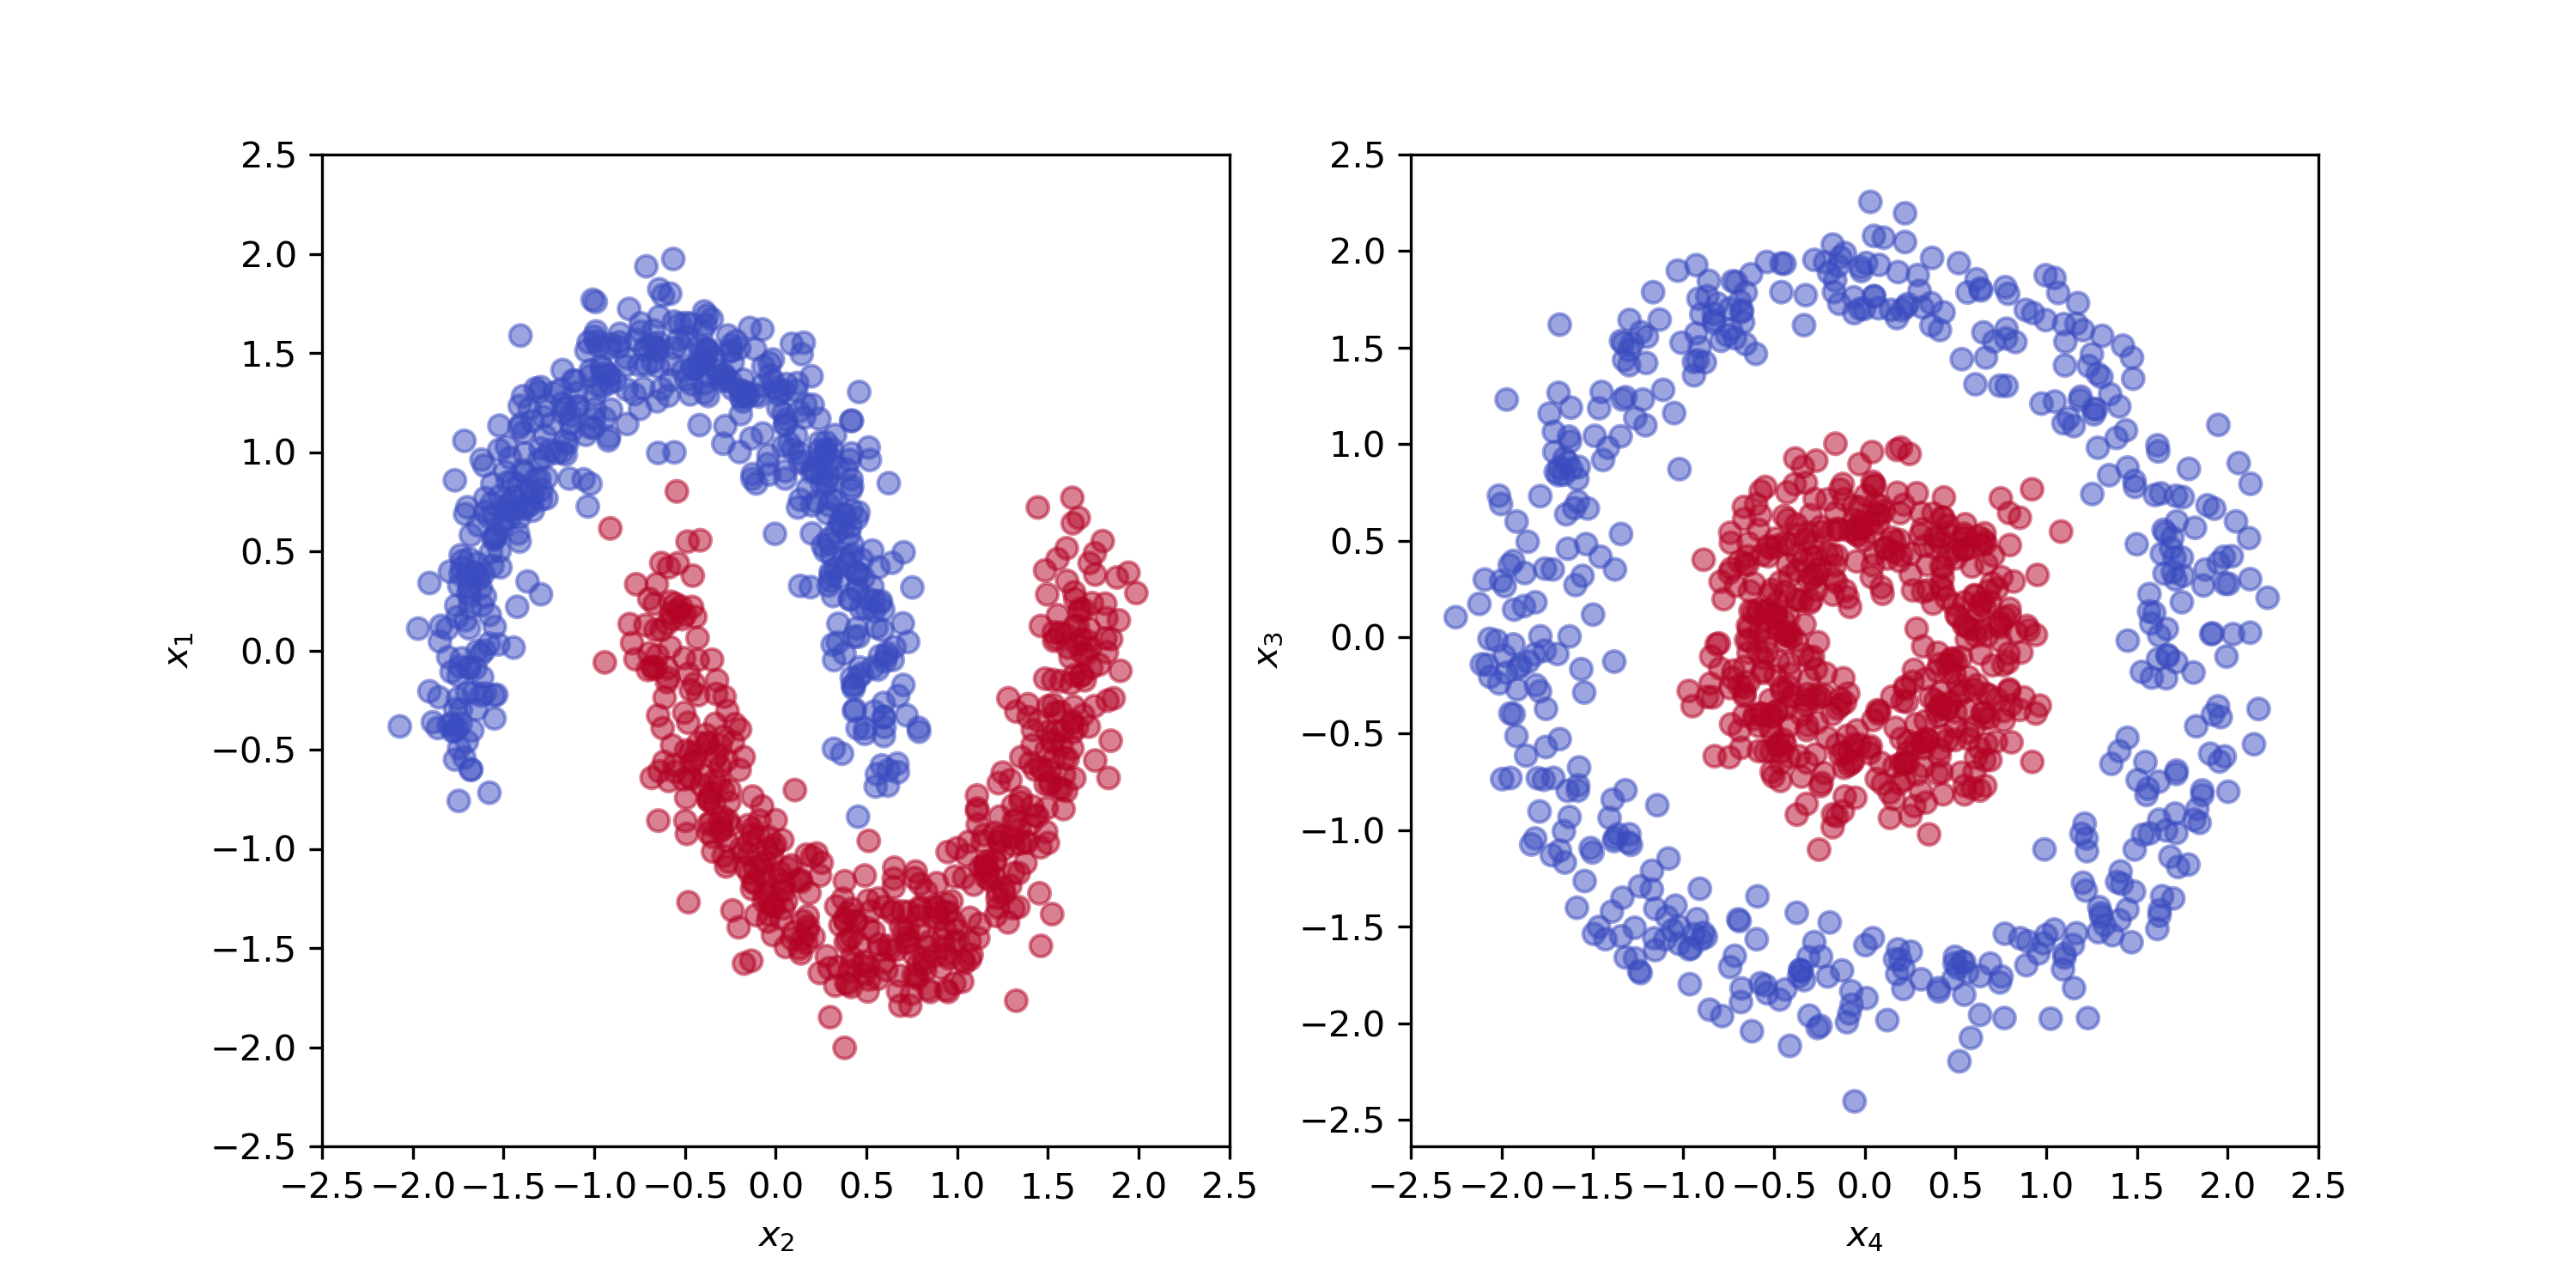
\includegraphics[width=1.0\linewidth]{moons-circles.png}
    \caption{
        The `Two Moons' dataset (left) and the `Circles' dataset (right), normalized. 
    }\label{fig:moons_circles}
\end{figure}

Concretley, let $( x_1 , x_2 )$ be the inputs of the two-moons dataset and $y_1 \in \{0,1\}$ the class label.
The data is generated by creating two half circles of evenly spaced points, with a radius of one.
One of the half circles is rotated by 180 degrees and shifted by $0.5$.
Gaussian noise with a mean of zero and standard deviation of $0.1$ is added to each point in the dataset.
Let $( x_3 , x_4 )$ be the inputs of the cirlces dataset and $y_2 \in \{0,1\}$ the class label.
The data is generated by creating evenly spaced points on the inner and outer circles. 
The center of both circles is at $(0,0)$ and the radius of the outer circle is one.
The radius of the inner circle is set to be $0.35$.
Gaussian noise with a mean of zero and standard deviation of $0.1$ is added to each point in the dataset.
The values of noise and the size of the inner circle are selected, such that the points do not mix among the circles.

\begin{figure}[ht]
\centering
\begin{minipage}{\linewidth}
\begin{lstlisting}[
    language=Python,
    captionpos=b, 
    label={code:data},
    caption={Generation of Moons-Circles dataset; pseudo code},
]
from sklearn import make_circles, make_moons
from sklearn.model_selection import train_test_split

# generates shuffled data points with labels
# x1, x2 -> shape=(1000, 2); y1, y2 -> shape=(1000, ) 
x1, y1 = make_circles(n_samples=2000, noise=0.1, factor=0.35)
x2, y2 = make_moons(n_samples=2000, noise=0.1)

circles_moons_x = concatenate(x1, x2) # shape=(1000,4)
circles_moons_y = concatenate(y1, y2) # shape=(1000,2)

# split the dataset in half
x_train, x_test, y_train, y_test = train_test_split(
    circles_moons_x, circles_moons_y, test_size=0.5
)

# scale data to zero mean, unit variance, based on training data
scaler = sklearn.preprocessing.StandardScaler().fit(x_train)
x_train = scaler.transform(x_train)
x_test = scaler.transform(x_test)

(x_train, y_train) # the training data
(x_test, y_test) # the test data
\end{lstlisting}
\end{minipage}
\end{figure}

The classic machine learning library `scikit-learn' is used to generate the data. 
The code snippet~\ref{code:data} outlines the generation process as Python-flavoured pseudo code.
The previously described sampling strategies for the data relate to the implementation in the `scikit-learn' Python library.
The data is generated with the \lstinline{makemoons}, and \lstinline{makecircles} functions, respectively.
Since the ranges of values of the datasets are different due to their sampling strategy, each feature is normalized individually to have zero mean and unit variance.
The final, normalized dataset is depicted in figure~\ref{fig:moons_circles}

To create a single dataset out of the two separate datasets, the input features as well as the labels are concatenated.
Concretely, one sample of the concatenated dataset $\hat x$ contains one randomly selected sample from the two moons dataset and one randomly selected sample from the circles dataset.
The label $\hat y$ of the sample $\hat x$ also consists of the respective concatenated labels.

\[\hat x = ( x_1 , x_2 , x_3 , x_4 )\]
\[\hat y = ( y_1 , y_2 )\]

In this way, the whole dataset is concatenated.
Afterward, the dataset is randomly split in half into a training set and a test set.
The result is a training set and a test set with 1000 samples each.
This dataset contains two separate and independent tasks.
For each task, only the respective inputs contain valuable information for the prediction of the class.

\begin{figure}[ht]
    \centering
    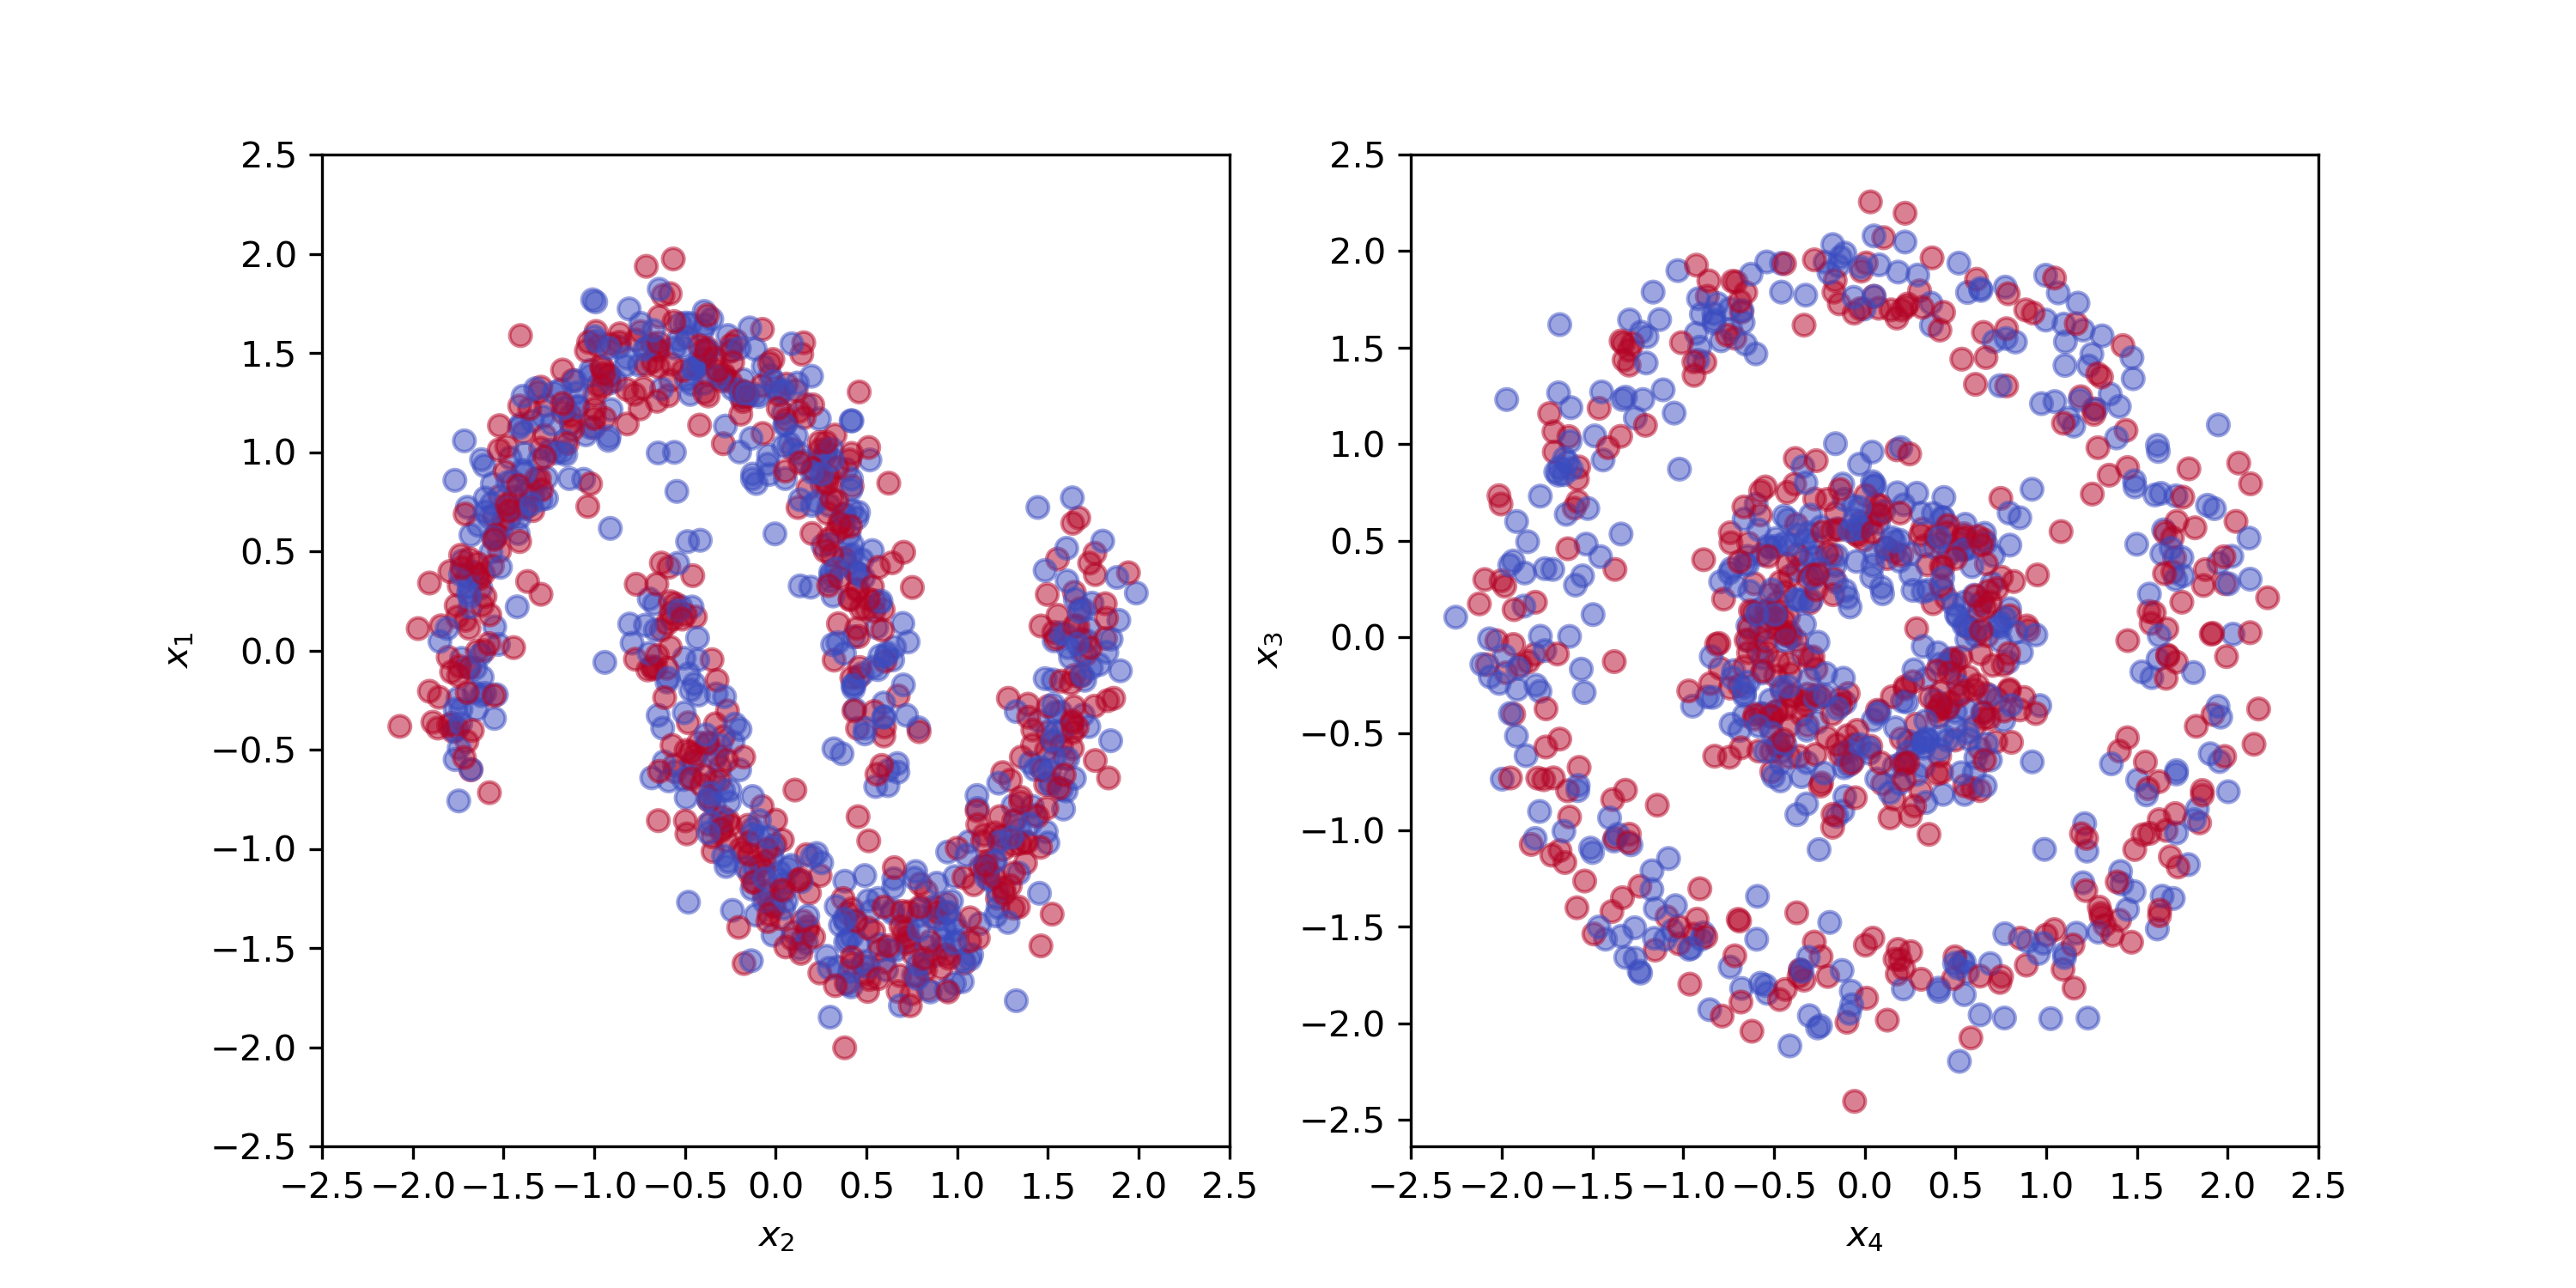
\includegraphics[width=1.0\linewidth]{moons-circles-inverted.png}
    \caption{
        The `Two Moons' dataset (left) with `Circles' labels, and the `Circles' dataset (right) with `Two-Moons' labels. 
    }\label{fig:moons_circles_inverted}
\end{figure}

The independence is demonstrated in figure~\ref{fig:moons_circles_inverted}.
The dataset is the same as is visible in figure~\ref{fig:moons_circles}. 
However, the Two-Moons dataset is displayed with the labels of the Circles dataset and vice versa.
Concretely, on the left side, the coordinates represent $x_1$ and $x_2$, but the colors refer to $y_2$.
On the right side on the other hand, $x_2$ and $x3$ are displayed with the colors defined by $y_1$.
There is no clear visible pattern discernible from these datasets given on their own.

The generation procedure of the datasets is outlined in the Python-flavoured pseudo code snippet~\ref{code:data}.
First, both datasets are individually generated.
The samples and labels are then concatenated into one dataset, which is then randomly split into the training and test set.
Finally, the data is normalized to zero mean and unit variance, based on the training set.

The generated dataset will be referred to as the `Moons-Circles' dataset.

\section{Network Architecture and Hyperparameters}
The neural network used to train on the `Moons-Circles' dataset was inspired by the original lottery ticket experiments by \textcite{LTH}. 
The neural network employed in the thesis consists of four input neurons, two output neurons, and a variable number of hidden layers ranging from one to three.
The experiments conducted throughout the thesis involve exploring different configurations of hidden layers.
The input neurons correspond to $x_1, x_2, x_3, x_4$ defined of the `Moons-Circles' dataset, defined in the previous paragraph~\ref{sec:independece_dataset}.
The network outputs correspond to the labes $y_1$ and $y_2$ of the datset.

As non-linearity, the Rectified Linear Unit (ReLU) is used.
The Gaussian Xavier-initialization~\textcite{XAVIER-GLOROT} was used by \textcite{LTH} in the original experiments.
However, the authors did not justify their decision and since the networks use the ReLU activation function, Gaussian Kaiming-initialization~\autocite{KAIMING-HE} will be used to initialize the weights.
The initialization of the biases is not mentioned by \textcite{LTH}.
Throughout this thesis the biases are initialized with zero.
The random initialization of the weights is explicitly controlled via a random seed, to enable reproducibility.
Throughout the thesis, experiments are repeated with three to five different seeds for the weight initialization to attain robust results.

The network simultaneously classifies two independent tasks.
Each of those tasks is a binary classification problem.
Therefore, the binary cross entropy is used as a loss function.
It is calculated for each task separately.
The total loss is calculated as the sum of the losses of each binary classification task. 

\section{Training Procedure}
With the dataset and architecture described above the goal is to find lottery tickets.
To accomplish this task, the classic iterative magnitude pruning algorithm described in paragraph~\ref{sec:lth}, which was used by \textcite{LTH} in the original lottery ticket experiments.
\textcite{LinearModeConnectivity} demonstrated that the LeNet architecture trained on MNIST is stable at initialization, meaning that lottery can be found rewinding the weights to  the value at initialization. 
Since the model and dataset in our case are significantly less complex, it is assumed that resetting the weights to their initial value is sufficient to discover lottery tickets.

The weights are pruned by magnitude as they are in the original lottery ticket experiments~\autocite{LTH}. 
Since \autocite{Supermasks} showed that magnitude pruning is amongst the best-performing criteria, it was selected due to its simplicity and widespread usage.
Biases are not pruned in the scope of this thesis.
Contrary to \autocite{LTH} where layerwise pruning is applied, the network is pruned globally in the following experiments..
Concretely, the pruning criterion is applied to all weights at once.
This enables the algorithm to `select' the sparsity for each layer on its own, resulting in fewer assumptions that have to be made.

Iterative magnitude pruning consists of several iterations, which are called `pruning levels'.
One pruning level includes training the network to convergence, pruning $p$-percent of the network and resetting the unpruned parameters to their values before training.
One complete run of iterative magnitude pruning, which includes all pruning levels, will be denoted a `training run'.
One training run consists of $L$ pruning levels.

At the beginning, all parameters of the network are unpruned.
After $L$ pruning levels, the `pruning target' is reached, which denotes the final number of unpruned parameters.
The sequence from the initial number of unpruned parameters to the pruning target is termed `parameter trajectory'.

The parameter trajectory is used to define the pruning part of the training run.
A parameter trajectory can be uniquely described by 3 out of the following 4 values:
\begin{itemize}
    \item initial number of parameters
    \item number of pruning levels, $L$
    \item pruning rate, $p$
    \item pruning target
\end{itemize}

Different combinations can be useful for different scenarios.
For example, for some experiments it is important that the networks have the same number of final parameters.
Then, it can be defined with the pruning target.
In a different scenario, the networks may need the same number of iterations and pruning rate, but the pruning target does not need to be fixed.

The networks are trained with the ADAM optimizer.
The learning rate is set to 0.001 and a batch size of 64 is used.
These values were selected based on their effectiveness in preliminary experiments. 
However, it is important to note that they are somewhat arbitrary and may be suboptimal.
Throughout the experiments, early stopping is used to reduce the computational time.
\textcite{LTH} used the early stopping iteration of the network on the LeNet architecture to indicate when the network converged.
Early stopping is implemented with a patience of 30 levels and the metric that is watched is the validation loss.
This means, that if the validation does not improve for 30 consecutive epochs, the training of the level is stopped and the next level is started.

As a pruning target for the experiments with the Moons-Circles dataset, values between 100 and 120 were selected.
The pruning target is, in many experiments, derived from the model architecture which will be described in detail in a later chapter.

\begin{minipage}{\linewidth}
\begin{lstlisting}[language=Python,caption={Iterative magnitude pruning with parameter resetting; pseudo code},captionpos=b, label={code:imp}]
model: torch.nn.module  # the freshly initialized model 
parameter_trajetory: List[int] # defines the pruning process
train_data, test_data  # data for training

# save state to reinitialize after pruning
initial_model_state = save_model_state(model)

parameter_count = parameter_trajetory[0]
for target in parameter_trajectory:
    if not first_iteration:
        pruning_amount = parameter_count - parameter_target
        parameter_count = parameter_target
        prune(model, pruning_amount)  # prune the model 
        reinit(model, initial_model_state)  # reinitialize the model

    # actual training and evaluation
    train_loss = train(model, train_data)
    val_loss, val_accuracy = evaluate(model, test_data)

    # transform to a graph and see if it split or degraded
    dag = transform_to_digraph(model)
    evaluate_dag(dag)

    # the run is stopped when graph is degraded 
    # to limit training time
    if graph_degraded: break

    # early stopping is used to limit training time
    if early_stopping(val_loss): break
\end{lstlisting}
\end{minipage}

In the code snippet~\ref{code:imp} the algorithm for iterative magnitude pruning is depicted in Python-flavoured pseudo code.
Details have been omitted for readability.
Importantly, the order of the commands is outlined to give a better sense of the algorithm.
The algorithm requires a neural network, parameter trajectory, and a dataset.
The \lstinline{model} refers to the freshly initialized neural network.
The parameter trajectory, as described earlier in this paragraph, refers to the number of unpruned parameters the network will have at every pruning level.
The difference between two neighboring entries in the parameter trajectory gives the number of parameters to prune at the given level.

\section{Finding Subnetworks}
The goal of the experiments is to show wether there are independent subnetworks in the network.
Therefore, a method to check wether this is the case needs to be defined.

Before the first pruning level, the network is converted into a directed acyclic graph $\mathcal{G}$.
This graph representation is maintained throughout the pruning levels and updated after each level.
To create the graph from a feed forward neural network, each neuron is converted to a node in the graph.
Each node is assigned a layer.
Each node in layer $i$ is connected to each node in layer $i+1$ with an edge.
Each edge is assigned the value of the weight that connects the two neurons.
All nodes, except for the input layer, have biases associated with them.
Because the network is pruned in an unstructured fashion (prune weights directly, not neurons), there is the possibility for node to have no incoming or outgoing edges.
To represent the different scenarios that nodes and edges can fall under, four categories are defined.

\begin{enumerate}
\item active parameters  \\
Nodes or edges in the graph that are connected to at least one input node and at least one output node.
\item inactive parameters \\
Nodes or edges that are not connected to any output node. They do not influence the result of the network and they do not receive gradients. They can be removed.
\item pruned parameters \\
Nodes or edges that have been masked out by the pruning algorithm.
\item zombie parameters \\
Nodes or edges that are not connected to any input node, but are connected to at least one output node.
\end{enumerate}

Before the first pruning level, all nodes and edges are classified as `active parameters'.
After the network was pruned, each parameter in the network is evaluated and assigned the correct category.

After a pruning level, the newly pruned weights are added to the `pruned parameters' category.
A subgraph $\mathcal{G}_{unpruned}$ is created, excluding all pruned weights.
On $\mathcal{G}_{unpruned}$, inactive nodes and edges are found and assigned their category.
All nodes that are not connected to any output node are classified as inactive.
Further, all edges that are connected to an inactive node are classified as inactive.

Then, a subgraph $\mathcal{G}_{active/zombies}$ is created, excluding all pruned and inactive weights.
On $\mathcal{G}_{active/zombies}$ zombie parameters are found and assigned to their category. 
All nodes that are not connected to any input feature are classified as a zombie parameter. 
Further, all edges that are connected to a zombie node are classified as a zombie parameter.

An active subgraph $\mathcal{G}_{active}$ is created, where all nodes have a path to at least one input node and at least one output node.
The active graph $\mathcal{G}_{active}$ is used to find separate components in the graph.

\begin{figure}[ht]
\centering
\begin{minipage}{\linewidth}
\begin{lstlisting}[
    language=Python,
    captionpos=b, 
    label={code:split},
    caption={
    Find independent subnetworks; pseudo code
    },
]
import torch
import networkx as nx

model: torch.nn.module  #  the neural network

# torch model -> networkx directed acyclic graph
G: nx.DiGraph = transform_to_digraph(model)

# remove pruned, inactive, and zombie parameters
G_unpruned = remove_pruned_parameters(G)
G_active_zombies = remove_inactive_parameters(G_unpruned)
G_active = remove_zombie_parameters(G_active_zombies)

# check for independent subgraphs in the active graph
subnetworks = []
for c in nx.connected_components(G_active.to_undirected()):
    subnetwork = G_active.subgraph(c)
    subnetworks.append(subnetwork)
\end{lstlisting}
\end{minipage}
\end{figure}

The code snippet~\ref{code:split} outlines the process of finding the subnetworks.
First, the PyTorch model is converted into a networkx graph.
As described previously, the active subgraph \lstinline{G_active} is created.
With the function \lstinline{connected_components}, components inside the graph that are not connected to each other are found.
Each node or edge of $\mathcal{G}_{active}$ is contained in exactly one of the subnetworks.
There is no overlap between the subnetworks.

\section{Matching Tasks to Subnetworks}\label{sec:taskmatch}
The subnetworks that are found with the methods described in the previous paragraph now must be matched with the tasks.
In order to check if the networks match the tasks, each task must be associated with certain input and output features of the data.
For each subnetwork and each task in the dataset, the inputs and outputs of the network are compared to the inputs and labels of the task.

Let $T$ be a task that has associated inputs and outputs.
The input features of the task are in the set $T_{in}$ and the output features in $T_{out}$.
Further, the input and output neurons of a network are referred to as $N_{in}$ and $N_{out}$ respectively.
For each network and each task, the amount to which the network covers the inputs or outputs of the task can be calculated.
Regarding the inputs, this quantity $C_{in}$ is referred to as input-coverage. The output-coverage is denoted as $C_{out}$.

The number of features that are covered by the network can be as the cardinality of the intersection of the network features and the task features $ |N \cap T|$, where  $|A|$ denotes the cardinality of set $A$.
To attain the coverage, the number of features covered by the network is divided by the number of features the task contains.
Then, the coverage is calculated for inputs and outputs as 

\[
c_{in} = \frac{|N_{in}  \cap T_{in} |}{|T_{in} |}
\]
\[
c_{out} = \frac{|N_{out}  \cap T_{out} |}{|T_{out}|}
\]

In a scenario where all inputs and all outputs are important, the combined input- and output-coverage might be considered.
The coverage should keep the characteristics of the input- and output-coverage, namely, that it is one when all features are covered, zero when no features are covered, and between one and zero if some but not all features are covered.
This can be achieved by multiplying the coverages.
Therefore, the overall coverage $c_{inout}$ is defined as:

\[
    c_{inout} = c_{in} * c_{out}
\]

A network is considered \textbf{separated} if and only if each of its subnetworks has coverage of exactly one and there are as many subnetworks as there are tasks.
If one of the subnetworks has coverage of less than one, the whole network is considered \textbf{degraded}, even though some other networks might cover the tasks perfectly.

Concretely, consider the dataset in paragraph~\ref{sec:independece_dataset}.
The overall coverage $c_{inout}$ is used since all inputs and outputs are essential for the network to function well.
It contains two tasks: the `Moons'-task and the `Circles'-task. 
The moons-task $T^{(1)}$ is associated with the inputs $T^{(1)}_{in} = \{x_1,x_2\}$ and the output $T^{(1)}_{out} = \{y_1\}$.
The circles-task $T^{(2)}$ is associated with the inputs $T^{(2)}_{in} = \{x_3,x_4\}$ and the output $T^{(1)}_{out} = \{y_4\}$.

The coverages can be collected in a matrix $C$ of size $J \times K$, where $J$ is the number of tasks and $K$ is the number of subnetworks. 
$c_{j,k}$ represents the value at the $i$-th row and the $j$-th column and $0 \leq c_{j,k} \leq 1$ holds.
The sum of the matrix is upper bound by the number of tasks.
\[
\sum^{i} \sum^{j} c_{j,k} \leq J
\]

Given an unpruned network and a dataset with two tasks the matrix would look like the following 
\[
C = \begin{pmatrix}
    1 \\ 1
\end{pmatrix}
\]
Each task would be completely covered by the same network.
Since the network per definition covers all tasks before the first pruning level, the matrix will be a unit vector with as many entries as there are tasks.

After several pruning iterations, the network might contain two disconnected subnetworks.
In this case, an additional row is added to the matrix.
For instance, let the subnetworks perfectly match the tasks such that every task is completely covered by one subnetwork.
The matrix $C$ might look like the following.
\[
C = \begin{pmatrix}
    1 & 0 \\ 0 & 1
\end{pmatrix}
\]
After further pruning the network, all the connections to one of the input nodes might be pruned.
Then, one of the subnetworks would not be completely covered anymore.
Assuming that the input feature $x_2$ of the `Moons'-task $T^{(1)}$ is completely disconnected, the input-coverage would be evaluated as 
\[
    c_{in} = \frac{|N_{in}  \cap T_{in} |}{|T_{in} |} = \frac{|\{x_1\} \cap \{x_1, x_2\}|}{|\{x_1, x_2\}|} = \frac{1}{2}
\]

and the resulting matrix $C$ would look like the following

\[
C = \begin{pmatrix}
    1 & 0 \\ 0 & 0.5
\end{pmatrix}
\]

If the sum of $C$ is equal to the number of tasks and the number of subnetworks is equal to the number of tasks, then the network is perfectly split.
If the sum of $C$ is equal to the number of tasks, but there are fewer subnetworks than tasks, the network still needs to split.
The number of splits that are required can be the difference between the number of tasks and the number of subnetworks.

If the sum of $C$ is less than the number of tasks, the network already has lost one input or output.
This scenario is referred to as a `degraded' network.
Once a network is degraded, a perfect separation cannot be reached anymore.
Generally, throughout this thesis, the training is stopped as soon as the network is degraded to save computational resources.

\section{Network Extension}\label{sec:extension}
Network extension is a technique used to create models that are comparable based on prunable parameters. 
First, the problem is described which model extension is intended to solve, then the technique is described in detail.

To compare networks over different pruning levels, a significant quantity is the number of prunable parameters the networks have left at each iteration.
For instance, comparing two networks with 1000 and 1200 prunable parameters in the beginning, 6 pruning levels, and a pruning rate of $0.2$, the following parameter trajectories $t_{1000}$ and $t_{1200}$ define the training.
\[
t_{1000} = [1000, 800, 640, 512, 409, 327, 262]
\]
\[
t_{1200} = [1200, 960, 768, 614, 491, 393, 314]
\]
Let $f_{1000}$ and $f_{1200}$ be the associated networks.
The first problem is that the pruning target is not aligned.
The final networks cannot be so easily compared, because they have different amounts of parameters available to them.
Therefore, let the pruning rate be variable. The pruning target is set to the same value for both networks.
The pruning rate can be calculated with 
\[
p = 1 - \sqrt[L]{\frac{T}{P}}
\]
where $L$ is the number of pruning levels, $P$ equals the number of prunable parameters before pruning and $T$ denotes the pruning target.

Let the pruning target be $200$ with 6 pruning levels.
The pruning rates are $p_{1000} = 0.235$ and $p_{1200} = 0.258$ respectively.
The resulting parameter trajectories are as follows.
\[
t_{1000} = [1000, 764, 584, 447, 341, 261, 200]
\]
\[
t_{1200} = [1200, 890, 660, 489, 363, 269, 200]
\]

With this change, the pruning targets are aligned and therefore, the final networks are comparable in a more fair way.
However, the number of available parameters is \textit{only} aligned at the very end.
Consider the following situation.
The network $f_{1000}$ separates after the fourth pruning level, where it has $341$ prunable parameters left. 
The other network $f_{1200}$ separates at iteration after the fifth level, where it has $269$.
At first glance, one could say that the network $f_{1000}$ was separated earlier.
It separated when it had more parameters available than the other network.
However, this misses part of the picture.
Given that the networks can only separate at the predefined trajectory, the network $f_{1200}$ would have had to separate at $363$ parameters.
Therefore, the $f_{1200}$ \textit{maybe would} seperate earlier than $f_{1000}$.
In the range of $363$ to $341$ where the $f_{1200}$ would have more parameters than $f_{1000}$, is not checked anymore.
This makes it hard to compare the networks during their pruning trajectory.
Especially regarding the pruning level when they split, as they cannot be compared fairly.
Ideally, different networks would have parameter trajectories that are shared, such that they can be compared at every step.

To achieve this, we will start with a small network which will be referred to as the base model.
Let the base model be a network with the shape $(4, 8, 8, 2)$.
This network has $112$ weights and $18$ biases.
To extend this network, a pruning rate $p$ must be defined.
The task now is to find a larger network, which will have the same number of unpruned parameters \textit{after} it was pruned with the defined pruning rate.

To extend the model now for one level, a new architecture has to be found, which, when pruned once with a pruning rate of $p=0.32$, has $112$ remaining parameters.
To extend the base model for two levels, the same method is used, but the resulting network must be pruned twice to reach the desired number of parameters, $112$ in this case.
To keep the task simple, the network architecture is restricted to a fixed number of hidden layers where each layer contains the same number of neurons.
Further, for the experiments in this thesis, only the weights are considered, since biases are not pruned.
However, the technique is easily extensible to take the biases into account.

Concretely, let $N$ be the number of weights in a network.
The equation to calculate the number of weights is given as follows

\begin{equation} \label{eq:num_params}
    d_h d_{in}+(m-1)d_h^2 + d_h d_{out} = N
\end{equation}

, where $d_{in}$ and $d_{out}$ refer to the input and output dimension respectively, $m$ to the number of hidden layers and
$d_h$ to the number of neurons per hidden layer.
For the base model with shape $(4, 8, 8, 2)$ the values are $d_h=8$, 
$d_{in}=4$, $d_{out}=2$ and $m=2$.
 
To extend the model with a given pruning rate $p=0.32$, the number of parameters is updated to a target value denoted $\hat N$.
The value $\hat N$ should have the property that, when pruned with a pruning rate of $p$, it should again be $N$.

Therefore, for one extension level:
\[
\hat N = {(\frac{N}{1-p})}
\]
And generalizing for any number of extension levels

\[
\hat N = {\frac{N}{{(1-p)}^L}}
\]
, where $L$ refers to the number of extension levels.

$\hat N$ now represents the target number of parameters. 
To find a network architecture that has this amount of parameters, one needs to insert $\hat N$ in the equation~\ref{eq:num_params}.
All parameters except for $d_h$ are set to a fixed value and the equation is solved for $d_h$.
Equation~\ref{eq:num_params} can be reformulated to a standard quadratic equation.

\[
    (m-1)d_h^2 + (d_{out} + d_{in}) d_h - \hat N = 0
\]
and therefore solved for $d_h$ with 
\[
    d_h = \frac{
        - d_{out} - d_{in} \pm \sqrt{  {(d_{out} + d_{in})}^2 + 4 \hat N (m-1) } 
    }{
        2(m-1)
    }
\]

The result of $d_h$ refers to the target number of hidden neurons in each layer.
However, it most likely is not an integer directly.
Therefore, the value is simply rounded to the nearest integer.

In the case of the network with $112$ weights and a pruning rate of $0.32$, $\hat N$ evaluates to $164.706$.
Entering $\hat N$ into the equation and solving for $d_h$, the two solutions are $d_h=10.1795$ and $d_h=-16.1795$.
Only positive solutions are of interest, therefore the second solution can be omitted.
Rounded to the nearest integer, the number of hidden neurons in each layer is set to $10$.

Through rounding the pruning rate is slightly different at every iteration.
This is generally the case when a pruning rate is given as a percentage since the number of weights that are pruned is always discrete.
In the previous example, the actual pruning rate would be calculated as follows:
The number of weights for the architecture extended by one level would be $160$.
The effective pruning rate is therefore $p_{eff}=1-\frac{112}{160}=0.3$.

A network can be extended an arbitrary number of times.
Importantly, the number of weights is fixed for each extension level.
The number of weights a network has at level one does not change, independent of the number of total extension levels.
Therefore, the networks share the same parameter trajectory as long as they are extended from the same base model with the same pruning rate.
This enables comparing networks of different sizes throughout all pruning levels they share.

\section{The MNIST-Fashion-MNIST Dataset}\label{sec:mnist}
To test the network splitting on a slightly more realistic problem, the MNIST-Fashion-MNIST dataset was created.
The dataset is created similarly to the Moons-Circles dataset described in paragraph~\ref{sec:independece_dataset}, but the MNIST dataset \autocite{mnist} and the fashion-mnist \autocite{fashion} dataset are used as tasks.
The MNIST dataset is a well-known dataset of handwritten digits. 
The training set consists of 60000 images and the test set of 10000.
It contains all digits from zero to nine in handwritten form, on a $28 \times 28$ pixel grayscale image.
This dataset was also used in the experiments original lottery ticket experiments \autocite{LTH}.

\begin{figure}[ht]
    \centering
    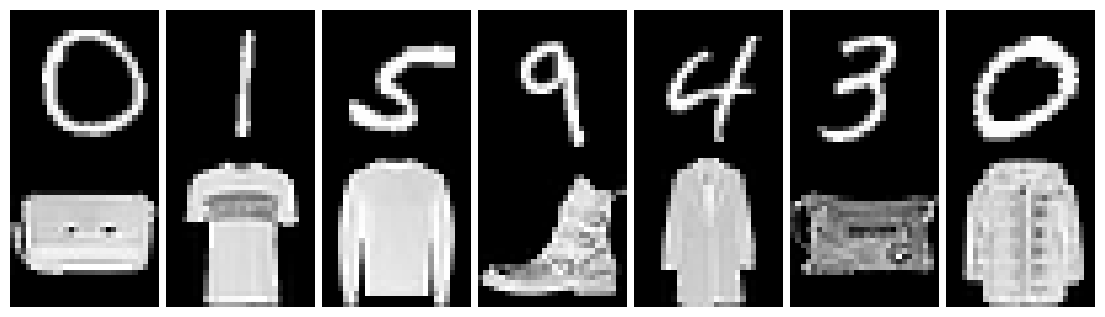
\includegraphics[width=1.0\linewidth]{mnist-fashion-mnist.png}
    \caption{
        MNIST-Fashion-MNIST dataset
    }\label{fig:mnist_fashion}
\end{figure}

As the name suggests, the fashion-MNIST dataset \autocite{fashion} is similar to the MNIST dataset.
However, instead of handwritten digits, different items of clothing are displayed on the $28 \times 28$ grayscale image.
It contains the same number of images for the test set and the training set.
Both datasets contain 10 classes.

In the same way as described in paragraph~\ref{sec:independece_dataset}, the datasets are concatenated into one.
Both datasets are shuffled and each sample from the MNIST dataset is concatenated with a random sample from the Fashion-MNIST dataset.
The class labels are also concatenated.
The result is a dataset with 60000 training samples and 1000 evaluation samples.
Through the concatenation, each image has an aspect ratio of $28 \times 56$, where each half corresponds to one of the datasets.
In figure~\ref{fig:mnist_fashion}, seven randomly selected samples of the  MNIST-Fashion-MNIST dataset are displayed.
On the top of each image, the handwritten MNIST digit is displayed. 
On the bottom the fashion item is visible.
Each sample consists of one random digit and one random fashion item. 

Contrary to the previous task, this dataset contains significantly more input features.
Each dataset has 784 input features, which results in 1586 input features for the concatenated dataset.
The Moons-Circles dataset only has four input features and two output features.
Further, the previous task was a combination of two binary classification tasks.
Now, each dataset represents a multiclass classification problem with 10 classes.

\subsubsection{Loss Function}
To enable training with this dataset, the loss has to be adapted.
For classification with more than two classes, the categorical cross entropy can be used.
For each of the tasks in the concatenated dataset, the loss is computed separately.
The total loss is simply the sum of the losses from each task.

Concretely, let $\mathbf{\hat y_{mnist}} = \left[\hat y_1, \dots, \hat y_{10}\right]$ be the output logits of the network that relates to the MNIST dataset and $\mathbf{\hat y_{fashion}} = \left[\hat y_{11}, \dots, \hat y_{20}\right]$ to the Fashion-MNIST dataset.
The labels are denoted fashion $\mathbf{y_{mnist}}$ and $\mathbf{y_{fashion}}$ respectively.
Together, they form the network output $\mathbf{\hat y} = \left[\hat y_1, \dots, \hat y_{20}\right]$

Let, $\mathcal{L} (\mathbf{\hat y}, \mathbf{y})$ be the loss of the network output $\mathbf{\hat y}$ and the true labels $\mathbf{y}$.
The total loss $\mathcal{L}$ of the network is calculated as follows:

\[
\mathcal{L}  (\mathbf{\hat y}, \mathbf{y})
= \ell  (\mathbf{\hat y_{mnist}}, \mathbf{y_{mnist}})
+ \ell (\mathbf{\hat y_{fashion}}, \mathbf{y_{fashion}})
\]

, where $\ell$ represents the categorical cross-entropy loss.

\subsubsection{Adapting Network Degradation}
In paragraph~\ref{sec:taskmatch} network separation and network degradation were introduced.
When trained on the Moons-Circles dataset from paragraph~\ref{sec:independece_dataset}, a network counts as degraded when any of the inputs or outputs are cut off from the network, since all inputs and outputs are relevant for the success of the network.
However, regarding the MNIST-Fashion-MNIST dataset, this is not the case.
Many of the input features do not carry information, for example, the outer frame of the MNIST images.
Therefore, it is to be expected that all connections to these inputs may be pruned.
This would likely lead to unwanted network degradation.

Therefore, the network only counts as degraded, if an output feature is completely cut off, meaning that it has no incoming connections anymore.
This requires only a small change in the calculation of the coverage as shown in paragraph~\ref{sec:taskmatch}.
The terms relating to the inputs of the tasks, namely $C_{in}$ and $T_{in}$, are simply to be exchanged for one.